\chapter{Deux modèles d'écoulement en milieu poreux : Darcy et Brinkman}

\noindent Les écoulements en milieu poreux sont modélisés par différentes lois. On choisit ici d'explorer les cas Darcy, première loi empirique obtenue et son extension à un terme visqueux, connu sous le nom de système de Brinkman. On étudie numériquement la dégénerescence du système de Brinkman en système de Darcy ; plus précisément, on pose la question de la robustesse du code face aux valeurs de la porosité du milieu.

\section{Description d'un milieu poreux}

Dans le cadre de ce mémoire, on caractérise un milieu poreux par sa porosité volumique, la dimension caractéristique de ses pores et par sa perméabilité associée. Il existe plusieurs types de milieux, selon la forme et l'organisation des pores en réseau et nous passerons ces points sous silence.

\paragraph{Volume d'un élément représentatif élémentaire} Le milieu poreux est un substrat solide présentant des trous, trous qui seront occupés par une ou plusieurs phases fluides. On définit en premier lieu la taille d'un volume élémentaire représentatif, de taille $l$, contenant plusieurs pores et des volumes fluides. On note alors $V := l^2$ pour des cellules carrées.

\paragraph{La porosité volumique} On note $\phi$ la porosité volumique d'un milieu poreux. Il est défini par le rapport entre les volumes de fluides sur volume d'un élément représentatif élémentaire. $$ \phi := \frac{V^f}{V} $$

\paragraph{La taille des pores} Les milieux diffèrent par la taille caractéristique des pores, par exemple, au sein d'un volume élémentaire représentatif, on peut associer la moyenne des longueurs de chaque élément solide ; on la note en général $d_p$ ou $d_f$ selon la forme des éléments solides.

\paragraph{La perméabilité du milieu} Enfin, on définit la perméabilité d'un milieu comme étant un tenseur dont les propriétés dépendent du milieu : il peut être réduit à un scalaire lorsque le milieu est isotrope, diagonal lorsque le milieu est orthotrope, ou plus généralement $$ \mathbf{K} := \begin{pmatrix} K_{xx} & K_{xy} \\ K{yx} & K_{yy} \end{pmatrix} $$ pour un milieu en deux dimensions en général. Le tenseur de perméabilité est fonction de la porosité $\phi$. La littérature fait essentiellement référence à deux lois de corrélation pour la perméabilité, on a pour les milieux granulaires dont le diamètre moyen d'une fibre est noté $d_p$
\begin{equation*} \tag{KC}
    K(\phi) \sim \frac{d_p^2 \phi^3}{180(1-\phi)^2} 
\end{equation*}
Cette loi est connue sous le nom de loi de Kozeny-Carman, introduite par Kozeny en 1927 et affinée par Carman en 1939. Une autre correspondant aux milieux fibreux, dont les fibres sont de taille $d_f$, organisés en réseau carré de cylindres parallèles et soumis à un écoulement parallèle, connue sous le nom de Happel-Langmuir (introduction en 1942 par Langmuir et étudiée par Happel en 1959)
\begin{equation*} \tag{HL}
    K(\phi) \sim \frac{d_f^2}{16(1-\phi)} \left( -\ln(1-\phi) - \frac{3}{2} + 2(1-\phi) - \frac{(1-\phi)^2}{2} \right)
\end{equation*}
Pour un réseau fibreux en deux dimensions, on dispose par exemple de la loi de Happel dont l'expression est
\begin{equation*} \tag{HL}
    K(\phi) \sim \frac{d_f^2}{32(1-\phi)} \left( -\ln(1-\phi) - \frac{1-(1-\phi)^2}{1+(1-\phi)^2} \right)
\end{equation*}
étudiée en 1959 toujours pas Happel.

\paragraph{Autres grandeurs} Si je n'ai présenté que les caractéristiques et lois utilisées ici, on trouvera d'autre nombres et lois servant à décrire la physique des écoulements en milieux poreux. La tortuosité par exemple, indice de la complexité du réseau de pores, les chaleur volumique et conductivité thermique pour étudier la thermodynamique, etc. On renvoie pour cela à \cite{jpc}.

\section{Dynamique des écoulements en milieu poreux}

\paragraph{Système de Darcy-Brinkman} On note toujours $\Omega$ un ouvert connexe borné lipschitzien de $\mathbb{R}^d$. L'équation décrivant un écoulement stationnaire d'un fluide newtonien incompressible dans un milieu poreux s'écrit sous la forme
\begin{equation*} \tag{B}
\begin{array}{rl}
    \nabla \cdot \mathbf{v} = & 0 \\
    -\tilde{\mu} \Delta \mathbf{v} + \mu \mathbf{K^{-1}} \cdot \mathbf{v} + \nabla p = & \rho \mathbf{f}
\end{array}
\end{equation*}
Ce genre de problèmes faisant apparaître un terme d'ordre 1 en vitesse est appelé problème de Stokes généralisé. On remarque que $\mu \mathbf{K}^{-1} > 0$ et on note ce coefficient $\alpha$. L'analyse du problème continu va à nouveau suivre le cours mentionné dans le chapitre précédent (cours de messieurs Frey et Privat). 

\paragraph{Formulation variationnelle} On note $V := H^1_0(\Omega)^d$ et $Q := L^2_0(\Omega)$, l'espace des fonctions de carré intégrable de moyenne nulle sur le domaine $\Omega$. La formulation variationnelle du système de Brinkman s'écrit

Trouver $\mathbf{v} \in V$, $p \in Q$,
\begin{align*}
    \int_\Omega (\alpha \mathbf{v} \mathbf{w} + \nabla \mathbf{v} : \nabla \mathbf{w}) dx - \int_\Omega p \nabla \cdot \mathbf{v} dx = & \int_\Omega \mathbf{f} \mathbf{w} dx \\
    \int_\Omega q \nabla \cdot \mathbf{v} dx = & 0
\end{align*}
$\forall \mathbf{w} \in V, q \in Q$. On définit les formes $$ a : V \times V \rightarrow \mathbb{R} \hspace{15pt} \mathbf{v}, \mathbf{w} \mapsto \int_\Omega (\alpha \mathbf{v} \mathbf{w} + \nabla \mathbf{v} : \nabla \mathbf{w}) dx $$ $$ b : V \times Q \rightarrow \mathbb{R}, \hspace{15pt} \mathbf{w}, q \mapsto - \int_\Omega q \nabla \cdot \mathbf{w} $$ et enfin $$ f : V \rightarrow \mathbb{R}, \hspace{15pt} \mathbf{w} \mapsto \int_\Omega \mathbf{f} \cdot \mathbf{w} dx $$ Le problème devient

Trouver $(\mathbf{v}, p) \in V \times Q$ :
\begin{align*}
    a(\mathbf{v}, \mathbf{w}) + b(\mathbf{w}, p) = & \mathbf{f}(\mathbf{w}) \hspace{10pt} \forall \mathbf{w} \in V \\
    b(\mathbf{v}, q) = & 0 \hspace{10pt} \forall q \in Q
\end{align*}

\begin{theoreme}
    Un couple $(\mathbf{v}, p)$ est solution du problème de Brinkman si, et seulement si, il est un point selle pour le lagrangien $$ \mathcal{L}(\mathbf{w}, q) := \frac{1}{2} a(\mathbf{w},\mathbf{w}) + b(\mathbf{w}, q) - f(\mathbf{w}) $$ donc si, et seulement si,
    $$ \mathcal{L}(\mathbf{v}, p) = \min_{\mathbf{w} \in V} \max_{q \in Q} \mathcal{L}(\mathbf{w}, q) $$
\end{theoreme}

\section{Expériences numériques pour le système de Brinkman dépendant du temps en deux dimensions}

\paragraph{Obtention du système linéaire} En notant $\mathbf{v} := \begin{pmatrix} u \\ v \end{pmatrix}$, le système de Brinkman dépendant du temps. En supposant que $\rho = 1$ et $\mu = 1$. Soit $\mathbf{K} = K \text{Id}_{\mathbb{R}^2}$. Le système de Brinkman en 2.D s'écrit

\begin{align*}
    \partial_x u + \partial_y v = 0 \\
    \frac{\rho}{\phi} \partial_t u -\frac{\mu}{\phi}\Delta u + \frac{\mu}{K} u + \partial_x p = f^u \\
    \frac{\rho}{\phi} \partial_t v -\frac{\mu}{\phi}\Delta v + \frac{1}{K} v + \partial_y p = f^v \\
    u_{|\partial \Omega} = u^D \\
    v_{|\partial \Omega} = v^D
\end{align*}

On utilise, comme pour le problème de Stokes, une méthode de projection scalaire sur maillage M.A.C. Le problème se construit à l'aide d'un tripler de Green-Taylor dépendant du temps, on considère les fonctions 
\begin{align*}
    u(t, x, y) = & sin(x)cos(y) e^{-2t} \\
    v(t, x, y) = & -cos(x)sin(y) e^{-2t} \\
    p(t, x, y) = & 0
\end{align*}

Dans ce cas le vecteur second membre s'écrit
\begin{align*}
    f^u(t, x, y) = \frac{1}{K} u(t, x, y) \\
    f^v(t, x, y) = \frac{1}{K} v(t, x, y)
\end{align*}

Le système linéaire de l'étape prédiction est donné par 
\begin{align*}
    \frac{\Delta y}{\Delta x} \left( \tilde{U}_{j,i+1} + \tilde{U}_{j, i-1} \right) + \frac{\Delta x}{\Delta y} \left( \tilde{U}_{j-1,i} + \tilde{U}_{j-1, i} \right) + \left[ 2\left( \frac{\Delta y}{\Delta x} + \frac{\Delta x}{\Delta y} \right) + (\Delta y \Delta x) \left(\frac{1}{\Delta t} + \frac{1}{K} \right) \right] \tilde{U}_{j,i} = \\ \Delta y \Delta x f^u_{j,i} + \frac{\Delta y \Delta x}{\Delta t} U_{j,i} - (\Delta y \Delta x) (P_{j,i} - P_{j, i-1}) \\
    \frac{\Delta y}{\Delta x} \left( \tilde{V}_{j,i+1} + \tilde{V}_{j, i-1} \right) + \frac{\Delta x}{\Delta y} \left( \tilde{V}_{j-1,i} + \tilde{V}_{j-1, i} \right) + \left[ 2\left( \frac{\Delta y}{\Delta x} + \frac{\Delta x}{\Delta y} \right) + (\Delta y \Delta x) \left(\frac{1}{\Delta t} + \frac{1}{K} \right) \right] \tilde{V}_{j,i} = \\ \Delta y \Delta x f^v_{j,i} + \frac{\Delta y \Delta x}{\Delta t} V_{j,i} - (\Delta y \Delta x) (P_{j,i} - P_{j-1, i})
\end{align*}

Ensuite on reconstruit la divergence sur le sous-maillage $\mathcal{T}^P$, avant d'implémenter le laplacien de Neumann moins un coin, qui aura la condition $\Phi_{0,0} = 0$.

Enfin, on peut corriger l'état via l'étape de correction :
\begin{align*}
    P^{(n+1)} = & \Phi + P^{(n)} \\
    U^{(n+1)} = & \tilde{U}^{(n+1)} - \Delta t \nabla_x \Phi \\
    V^{(n+1)} = & \tilde{V}^{(n+1)} - \Delta t \nabla_y \Phi
\end{align*}

On assemble le système pour les solutions de Taylor-Green. 

\paragraph{Tenseur de perméabilité sphérique} On suppose dans cette simulation que $\mathbf{K} := K \text{Id}_{\mathbb{R}^2}$. On étudie la convergence $L^2(\Omega)$ pour plusieurs discrétisations temporelles.
\begin{figure}[htp]
    \centering
    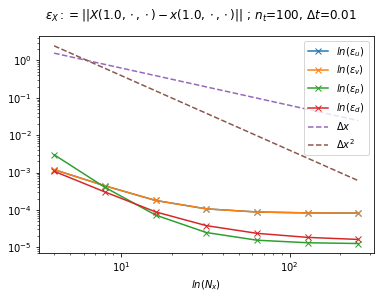
\includegraphics[width=7.5cm]{Images/brinkman/spherique/erreurs (2).png}
    \caption{Analyse de la méthode S.I.P jusqu'à $256 \times 256$ volumes.}
\end{figure}

\begin{figure}[htp]
    \centering
    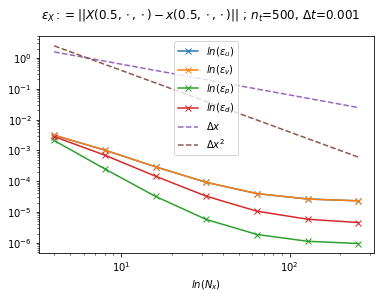
\includegraphics[width=7.5cm]{Images/brinkman/spherique/erreurs (3).png}
    \caption{Analyse de la méthode S.I.P jusqu'à $256 \times 256$ volumes.}
\end{figure}

\begin{figure}[htp]
    \centering
    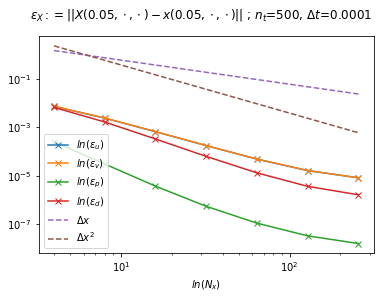
\includegraphics[width=7.5cm]{Images/brinkman/spherique/erreurs (4).png}
    \caption{Analyse de la méthode S.I.P jusqu'à $256 \times 256$ volumes.}
\end{figure}

\begin{figure}[htp]
    \centering
    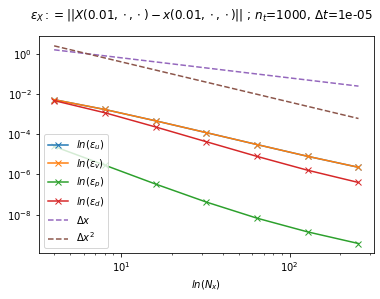
\includegraphics[width=7.5cm]{Images/brinkman/spherique/erreurs (5).png}
    \caption{Analyse de la méthode S.I.P jusqu'à $256 \times 256$ volumes.}
\end{figure}

\newpage

\paragraph{Tenseur de perméabilité orthotrope} On suppose cette fois que le tenseur $\mathbf{K}$ est diagonal de valeurs propres différentes. On prend un rapport de 1 à 5 et on constate que les erreurs des composantes de vitesse décoïncident, en norme $L^2(\Omega)$.
\begin{figure}[htp]
    \centering
    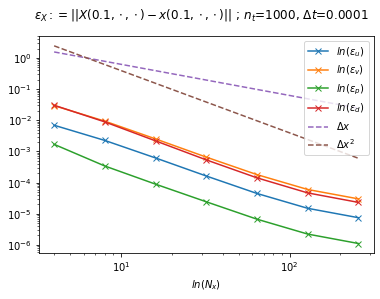
\includegraphics[width=7.5cm]{Images/brinkman/elliptique/erreurs (6), Kxx = .01, Kyy = .05.png}
    \caption{Simulation de Brinkman - Taylor - Green avec $\mathbf{K} := \begin{pmatrix} 0.01 & 0. \\ 0. & 0.05 \end{pmatrix}$ ; analyse jusqu'à $256\times 256$ volumes}
\end{figure}

\section{\'Etude numérique de la dégénerescence en système de Darcy}

Le système de Brinkman adimensioné fait apparaître le nombre de Darcy $$ Da := \frac{K}{L^2} $$ où $K$ est la hauteur de la cavité. On définit en général le nombre de Brinkman comme témoin du rapport entre le terme visqueux et le terme de Dacy. $$ Br := \frac{Da(\phi)}{\phi} $$

\paragraph{Estimation du nombre de brinkman en fonction de la porosité}

\newpage

\begin{figure}[htp]
    \centering
    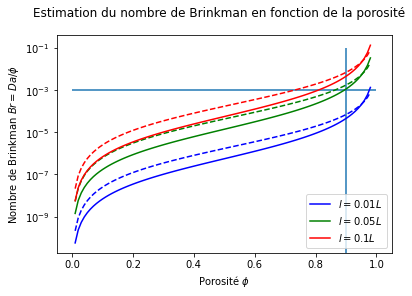
\includegraphics[width=7.5cm]{Images/brinkman/brinkman/brinkman.png}
    \caption{En pointillé : loi de Happel, en traits pleins : loi de Kozeny-Carman.}
\end{figure}

On voit que le rapport dépasse $10^{-3}$ pour les porosités supérieures à $0.9$ (courbe verte, cas Kozeny-Carman). Dans ce même cas, il est supérieur à $10^{-2}$ pour les porosités supérieurs à $0.95$. Cela donne une idée de la plage de valeurs sur laquelle le terme de Brinkman (visqueux) est négligeable devant le terme de Darcy, le terme d'inertie.

\paragraph{Robustesse du code} Une question intéressante est alors d'obtenir une idée de l'évolution de l'erreur, à discrétisation constante, en fonction de la porosité $\phi$. On déroule l'algorithme à discrétisation temporelle fixée, pour différents maillages entre $32 \times 32$ et $512 \times 512$, on obtient les courbes

\begin{figure}[htp]
    \centering
    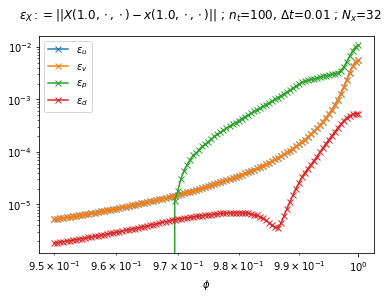
\includegraphics[width=7.5cm]{Images/brinkman/porosite/32.png}
    \caption{Zoom sur la plage $\phi > 0.95$}
\end{figure}

\begin{figure}[htp]
    \centering
    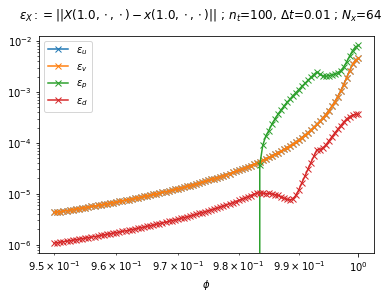
\includegraphics[width=7.5cm]{Images/brinkman/porosite/64.png}
    \caption{Zoom sur la plage $\phi > 0.95$}
\end{figure}

\begin{figure}[htp]
    \centering
    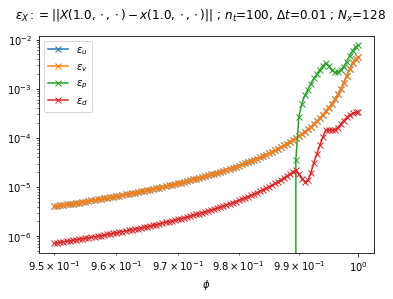
\includegraphics[width=7.5cm]{Images/brinkman/porosite/128.png}
    \caption{Zoom sur la plage $\phi > 0.95$}
\end{figure}

\begin{figure}[htp]
    \centering
    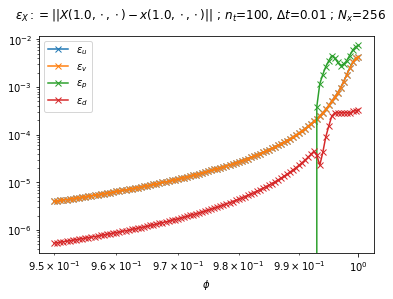
\includegraphics[width=7.5cm]{Images/brinkman/porosite/256.png}
    \caption{Zoom sur la plage $\phi > 0.95$}
\end{figure}

\begin{figure}[htp]
    \centering
    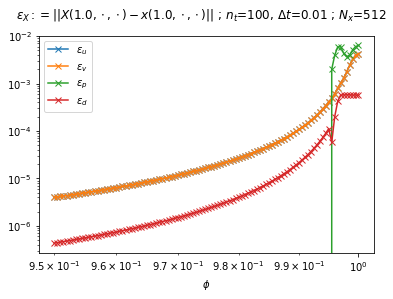
\includegraphics[width=7.5cm]{Images/brinkman/porosite/512.png}
    \caption{Zoom sur la plage $\phi > 0.95$}
\end{figure}

\newpage 

Quel que soit le maillage, il n'y a pas d'événement marquant avant les valeurs de porosité supérieures à $0.95$. En témoin de la tendance, les deux courbes qui montrent la croissance sur les plages $\phi \in [.1, .9]$ puis $\phi \in [.9, .94]$ :
\begin{figure}[htp]
    \centering
    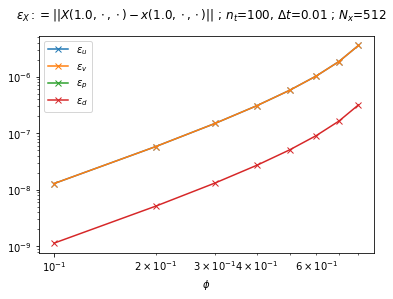
\includegraphics[width=7.5cm]{Images/brinkman/porosite/Figure 2021-11-20 180634 (21).png}
    \caption{Zoom sur la plage $\phi \in [.1, .9]$}
\end{figure}

\begin{figure}[htp]
    \centering
    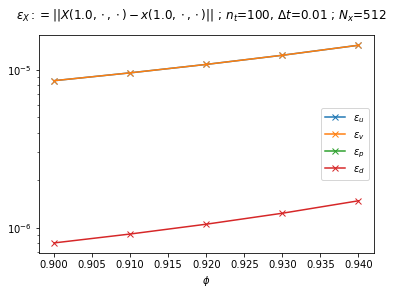
\includegraphics[width=7.5cm]{Images/brinkman/porosite/Figure 2021-11-20 180634 (22).png}
    \caption{Zoom sur la plage $\phi \in [.9, .95]$}
\end{figure}

\newpage

\section{Conclusion}

Dans ce chapitre, nous avons appris quelques éléments de modélisation des écoulements en milieux poreux, on a validé un code pour la simulation de ces écoulements et nous avons testé numériquement la limite de l'algorithme pour les grandes valeurs de $\phi$. On a également pu étudier la prépondérance du terme d'inertie, de Darcy, sur le terme visqueux, de Brinkman. \'A ce stade du mémoire, nous disposons donc d'un outil pour attaquer le problème de l'interface entre deux régions : une fluide, et une poreuse, séparées par une interface.